\documentclass {CSEThesis}
% Standard packages
\usepackage{amsmath}        % Extra math definitions
\usepackage{graphicx}       % PostScript figures
\usepackage{setspace}       % 1.5 spacing
%\usepackage{psfig,epsfig}
\usepackage{float}
\usepackage{multicol}
\usepackage{booktabs}
\usepackage{subfigure}
\usepackage{epsfig,color}
% Custom packages
%\usepackage[first]{datestamp}   % Datestamp on first page of each chapter

\usepackage{color}
%===== page layout
% Define the side margins for a right-side page
%\insidemargin = 1.3in \outsidemargin = 0.9in
% Above margin is space above the header
% Below margin is space below footer
%\abovemargin = 1.5in \belowmargin = 0.05in
\graphicspath{ {figures/} }

\btptitle = {Implementation of Speech Recognition System for Mobile Phones}
\name = {Abhinav Singh}
\rollno = {140101002}
\email = {abhinav.2014@iitg.ernet.in}
\guide = {Prof. Pradip K. Das}

\begin{document}

\begin{titlepage}
\begin{center}
\textheight 15.5in \textwidth 12.5in {\large\sf  \textbf{\the\btptitle}}\\[12ex]
{\small{\textsl{ \textbf{A B. Tech Project Report Submitted \\
in Partial Fulfillment of the Requirements \\
for the Degree of
\\[3ex]\small \bf Bachelor of Technology}}}}\\[16ex] \emph{by} \\[2ex]
{\sf \sf \textbf{\the\name}\\
             (\the\rollno)}\\[1ex]
\emph{under the guidance of}\\[2ex]
{\sf \bf \the\guide} \\[7ex]

\vspace{1.2in}

\begin{figure}[!h]
\hfill

\psfig{file=iitglogo.eps,width=0.15\textwidth} \hfill \
\end{figure}

{\sl \bf{to the}} \\[1ex]

{\small\bf DEPARTMENT OF COMPUTER SCIENCE AND ENGINEERING}  \\[1ex]
{\small \bf{INDIAN INSTITUTE OF TECHNOLOGY GUWAHATI \\GUWAHATI - 781039, ASSAM}}
%\\[2ex]
%
%  {\color{red} \hrule height 0.5ex}
% \vskip 1ex
% May \the\year 
\end{center}
\end{titlepage}

\newpage
\raggedbottom
\doublespacing
\pagenumbering{roman}

\chapter*{\centering \underline{CERTIFICATE}}
\vskip 2ex

\emph{\quad This is to certify that the work contained in this thesis titled ``\textbf{\the\btptitle}'' is a bonafide work of \textbf{\the\name} (\textbf{Roll No. \the\rollno}), carried out in the Department of Computer Science and Engineering, Indian Institute of Technology Guwahati under my supervision and that it has not been submitted elsewhere for a degree.}

\vskip 15ex
\begin{flushright}

Supervisor: \textbf{\the\guide}\\
\end{flushright}
~~~~~~~~~~~~~~~~~~~~~~~~~~~~~~~~~~~~~~~~~~~~~~~~~~~~~~~~~~~~~~~~~~~~~~~~~~~~~~~~~~~~~~~~~~~~~~~~~~~~~~~~~~~~~~~~~Professor\\ November, \the\year~~~~~~~~~~~~~~~~~~~~~~~~~~~~~~~~~~~~~ Department of Computer Science $\&$ Engineering\\ Guwahati~~~~~~~~~~~~~~~~~~~~~~~~~~~~~~~~~~~~~~~~~~ Indian Institute of Technology Guwahati, Assam
\newpage
\chapter*{\centering Acknowledgements}

\quad Foremost, I would like to  express my sincere gratitude to my supervisor \text{\the\guide}, for his continuous support, enthusiasm and immense knowledge. He has always guided and motivated me towards the completion of my work despite his busy schedule.

I also take this opportunity to thank my mentor Parabattina Bhagath P for his consistent assistance and the Department of Computer Science and Engineering, IIT Guwahati for providing me the facilities that were essential to carry out my project.
\newpage
\chapter*{\centering Abstract}

\textit{\quad Automatic speech recognition systems are an integral part of every voice-based assistant. Voice centric interfaces have become widely available with the evolution of mobile phones. Advancements in speech recognition algorithms, increased computational power and networking capacities have enabled this growth. Its applications include but are not limited to dialing, web search, and dictation of text messages. In this work, we implement a light-weight embedded speech recognition system using phoneme segmentation, linear predictive coding and template matching. We have taken a dataset of digits spoken in moderately quiet environment. The results indicate that the proposed system is able to identify the spoken digits with over 75\% accuracy.}

\tableofcontents 
\addcontentsline{toc}{chapter}{List of Figures} 
\listoffigures 
\addcontentsline{toc}{chapter}{List of Tables} 
\listoftables
\pagenumbering{arabic}
\def\headrulehook{\color{black}}      % Color the header rule

\chapter{Introduction}
\pagenumbering{arabic}\hspace{3mm}

Mobile users desire devices that they can control without much physical interaction. Applications like Siri are steadily gaining popularity with their hands free features. They can send data over to servers where sophisticated algorithms provide exceptionally accurate recognition results.
However in countries like India, where over 75 percent of the population has no internet, these applications are not suitable. Privacy is also a concern as these systems can share voice data with third parties. While open-source embedded systems like PocketSphinx are present, they require large amounts of training data which is usually not available for unpopular languages and is hard to collect and annotate.

In this work, we aim to implement a portable word based embedded speech recognition system for mobile phones, along with a graphics user interface for training on desktop, and a demonstrative voice controlled assistant for android. In chapter \ref{ch:survey}, we discuss a few related works and technologies of the proposed system. In chapter \ref{ch:proposal} we present the design and implementation of the proposed systems. In chapter \ref{ch:experiment} we discuss the expermients performed and their observations. Finally, we draw out conclusions and discuss the future work in chapter \ref{ch:conclusion}. In the appendix, we provide details of the assumed knowledge.
\chapter{Related Works and Technologies} \label{ch:survey}

\section{Speech Feature Extraction}
\cite{1327109} investigate various feature extraction techniques - MFCC, LPCC, PLP for speech recognition on mobile phones. Their study shows that MFCC features give the most accurate result. In 
\cite{divya} a review of the latest feature extraction techniques is done. In this work, various advantages and disadvantages of techniques like RASTA and PLDA are pointed out. 

\section{Speech Modeling Techniques}
\cite{Mustafa2017} presents a comparative analysis of Hidden Markov Model, Multi-Layer Perceptron, and Dynamic Multi-Layer Perceptron. They conclude that DMLPs are infeasible on mobile phones, while HMMs are the most accurate, and MLPs are the fastest. With the increase in size of the vocabulary, the execution performance of HMM suffers. \cite{10.1007/978-981-10-3920-1_46} talks about implementing a lightweight speech recognition system using HMMs for Gujarati language and achieves 87\% accuracy.

\section{Distance Measures}
Cepstral coefficients are widely used in speech recognition. Various distortion methods have been applied to find the distance between two coefficients. \cite{1165058} brings out a novel distance measure, the Tohkura distance - a weighted distance that outperforms Itakura distance and Euclidean distance. It also mentions a more accurate Mahalanobis distance and the main difficulties for applying it to speech recognition.

\section{Native Development on Android}
\cite{5600170} discusses a new component development approach by using Java Native Interface technology. The Native Development Kit (NDK) is a set of tools that allows writing native code for Android in C++. Speech processing and recognition requires fine grain control over memory management and speed, hence NDK is preferred over Dalvik Virtual Machine. C and C++ libraries act as the glue code while the frontends can be written with Java or Swift.

\section{Network Speech Recognition}
In this mode of speech recognition, the feature extraction and recognition are both delegated to the network server. The server is capable of doing complex computation and returns extremely accurate results. One of the major constraints of this mode is the dependence on telephone network and the performance degradation caused by low bit rate codecs, which becomes severe in the presence of transmission errors \cite{Kumar_rethinkingspeech}.
\chapter{Design and Implementation} \label{ch:proposal}

\section{Speech Recognition Library}

The library is written in C++11 for its performance, familiarity and wide spread adoption including on android, iOS, and desktops. 
C++11 and later versions provide smart pointers and a standard threading library which is important for portability. To aid building the library across various platforms, the CMake build system is used.

The speech recognition system works as given in the following flowchart:

\begin{figure}[h!]
    \centering
    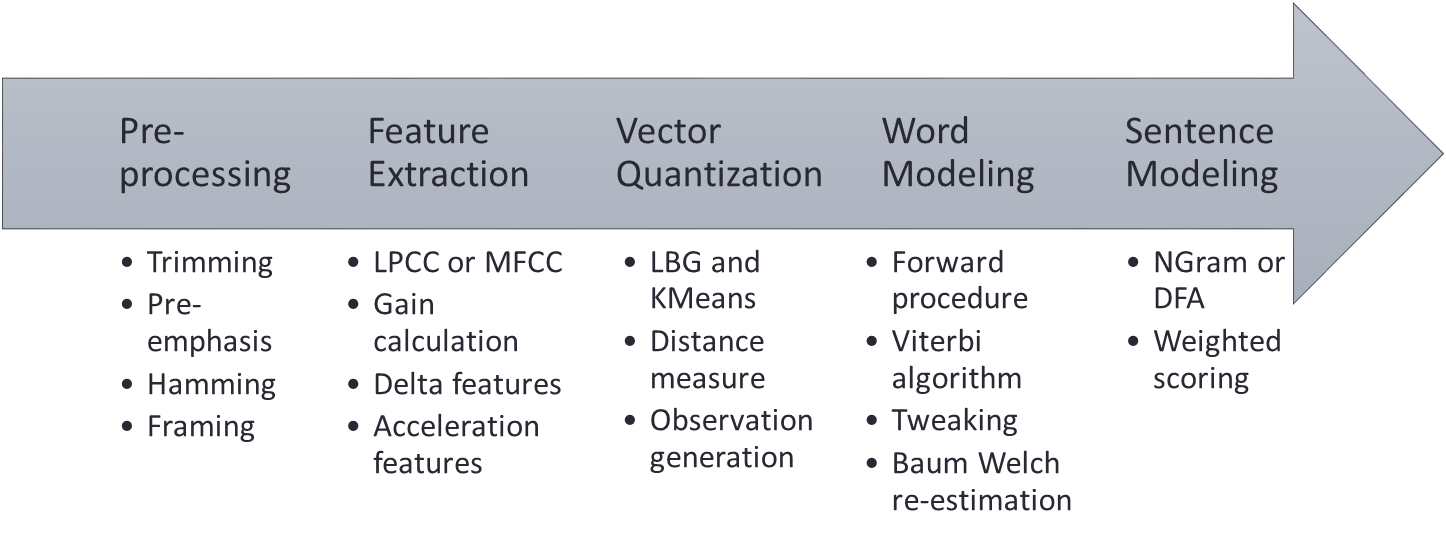
\includegraphics[scale=0.45]{training-flowchart}
    \label{fig:training-flowchart}
    \caption{Process flowchart}
\end{figure}

\subsubsection{Pre-processing}
The input signal is normalized and then trimmed using the algorithm described in \cite{Saha_anew}, which uses probability density function of the background noise to find boundaries. The resulting signal is divided into frames.

\subsubsection{Feature Extraction}
We have selected the features using the analysis in \cite{divya}. For each frame, Mel Frequency or Linear Predictive cepstral coefficients are generated. Cooley Tukey decimation algorithm is used for computing FFT and autocorrelation method is used for computing LPC. Finally, derivate coefficients are calculated using linear regression and added to the feature set.

\subsubsection{Vector Quantization}
Using LBG algorithm, the codebook is generated from the feature universe. This vastly reduces the data that has to be processed. Euclidean distance measure has been used to compare two feature vectors.

\subsubsection{Word Modeling}
Performed using Hidden Markov Models that have superior accuracy \cite{Mustafa2017} even in small vocabulary systems \cite{10.1007/978-981-10-3920-1_46}. Best path optimization using Baum Welch re-estimation is done to train the models, and forward procedure is used to test a model with the given input utterance. These methods are implemented with appropriate scaling and tweaking so they can work with limited floating-point precision.

\subsubsection{Sentence Modeling}
Performed by saving the counts of different sequences in the sentence list. Using these counts, NGram or DFA approach (for sentences that need to have a sequential ordering like commands) are implemented.

For training, HMM models are generated for each word by optimizing on all available word utterances in the training data. Sentence models are generated by parsing the given sentence list. Various parameters of this process can be changed using the configuration file. The graphical user interface can be used to simplify this process.

For testing, a sentence is input as a combination of words. For each word A in the sentence and for each word B in the training data, following steps are taken:

\begin{itemize}
\item Using HMM model of B, find probability of A matching B.
\item Using sentence models, find probability of occurrence of B given A’s position in the input sentence.
\item Final score is a linear combination of these two scores.
\end{itemize}

The word B with maximum final score is the best possible recognition. If its score is lesser than a cutoff score, then A is considered a null utterance, else B is returned.

The appendix describes the stages of this process in good detail along with code implementation examples.

\newpage

The library is written such that its clients do not have to dive deep into the technicalities of speech recognition. It has been divided into two abstraction layers:

\begin{enumerate}

\item Base

Provides implementation of various algorithms and techniques - Preprocessing, LPCC, MFCC, Derivative features, KMeans, LBG, HMM, NGram. Data objects - Codebook, Feature, Model, Gram are also described in this layer.

\begin{figure}[h!]
    \centering
    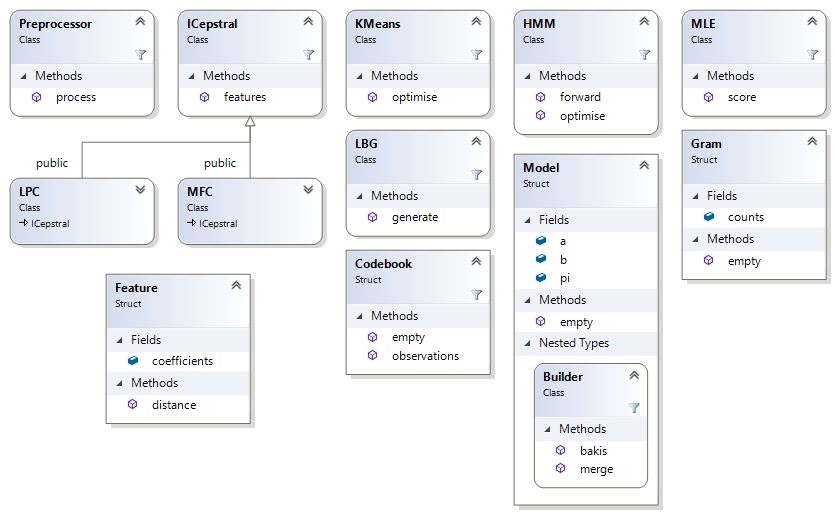
\includegraphics[scale=0.8]{sr-lib-base}
    \label{fig:sr-lib-base}
    \caption{Architecture of Base}
\end{figure}

This layer is not parallelized and strictly does not interact with the input/output e.g. WAV audio or saving/loading the data objects to the file system.

\newpage 

\item Word

Provides training and testing interfaces. The clients of the library are only allowed to interact with this layer.
This layer foresees construction and testing of HMM and NGram models. It implements handling inputs - WAV audio files, word list, sentence list, etc. It also implements functions to save and read generated data objects to and from the file system.

\begin{figure}[h!]
    \centering
    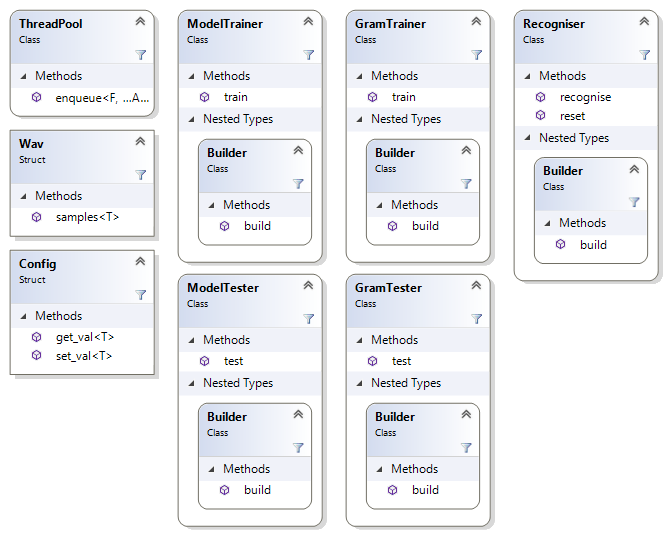
\includegraphics[scale=0.8]{sr-lib-word}
    \label{fig:sr-lib-word}
    \caption{Architecture of Word}
\end{figure}

This layer also handles the parallelization and configuration of the library.

The following tasks are parallelized:
\begin{itemize}
    \item Feature generation of multiple utterances
    \item Generation of multiple word models using HMM
    \item Matching of the input utterance with multiple word models
\end{itemize}

\begin{table}[h!]
    \centering
    \begin{tabular}{lll}
        Key          & Type &    Description \\ \hline
        q\_cache     & bool &    whether cached training files should be used \\
        n\_thread    & int &     number of threads used for parallel execution \\
        q\_trim      & bool &    whether the samples should be trimmed for background noise \\
        x\_frame     & int &     number of samples in a frame \\
        x\_overlap   & int &     number of samples to be overlapped while framing \\
        cepstra     & string &   mfc or lpc variants of feature generation \\
        n\_cepstra   & int &     number of features \\
        n\_predict   & int &     P of autocorrelation, only for lpc \\
        q\_gain      & bool &    whether gain term should be added to features \\
        q\_delta     & bool &    whether delta terms should be added to features \\
        q\_accel     & bool &    whether accel terms should be added to features \\
        x\_codebook  & int &     size of codebook \\
        n\_state     & int &     number of states in HMM \\
        n\_bakis     & int &     connectedness of initial bakis model for HMM \\
        n\_retrain   & int &     number of times each model should be trained \\
        n\_gram      & int &     number of previous words to be considered for prediction \\
        q\_dfa       & bool &    command based word prediction or probability based \\
        gram\_weight & double &  linear weight for the final scoring with recognition result \\
        cutoff\_score & double &  cutoff for final score \\
    \end{tabular}
    \caption{Keys for the configuration}
\end{table}

\end{enumerate}

\section{Graphical User Interface for Training}

The desktop graphical user interface is written in Swing Java framework. The interface can be run on Windows or Linux based OSes. It uses the Java Native Interface (JNI) for communicating with the speech recognition library.

\begin{figure}[h!]
    \centering
    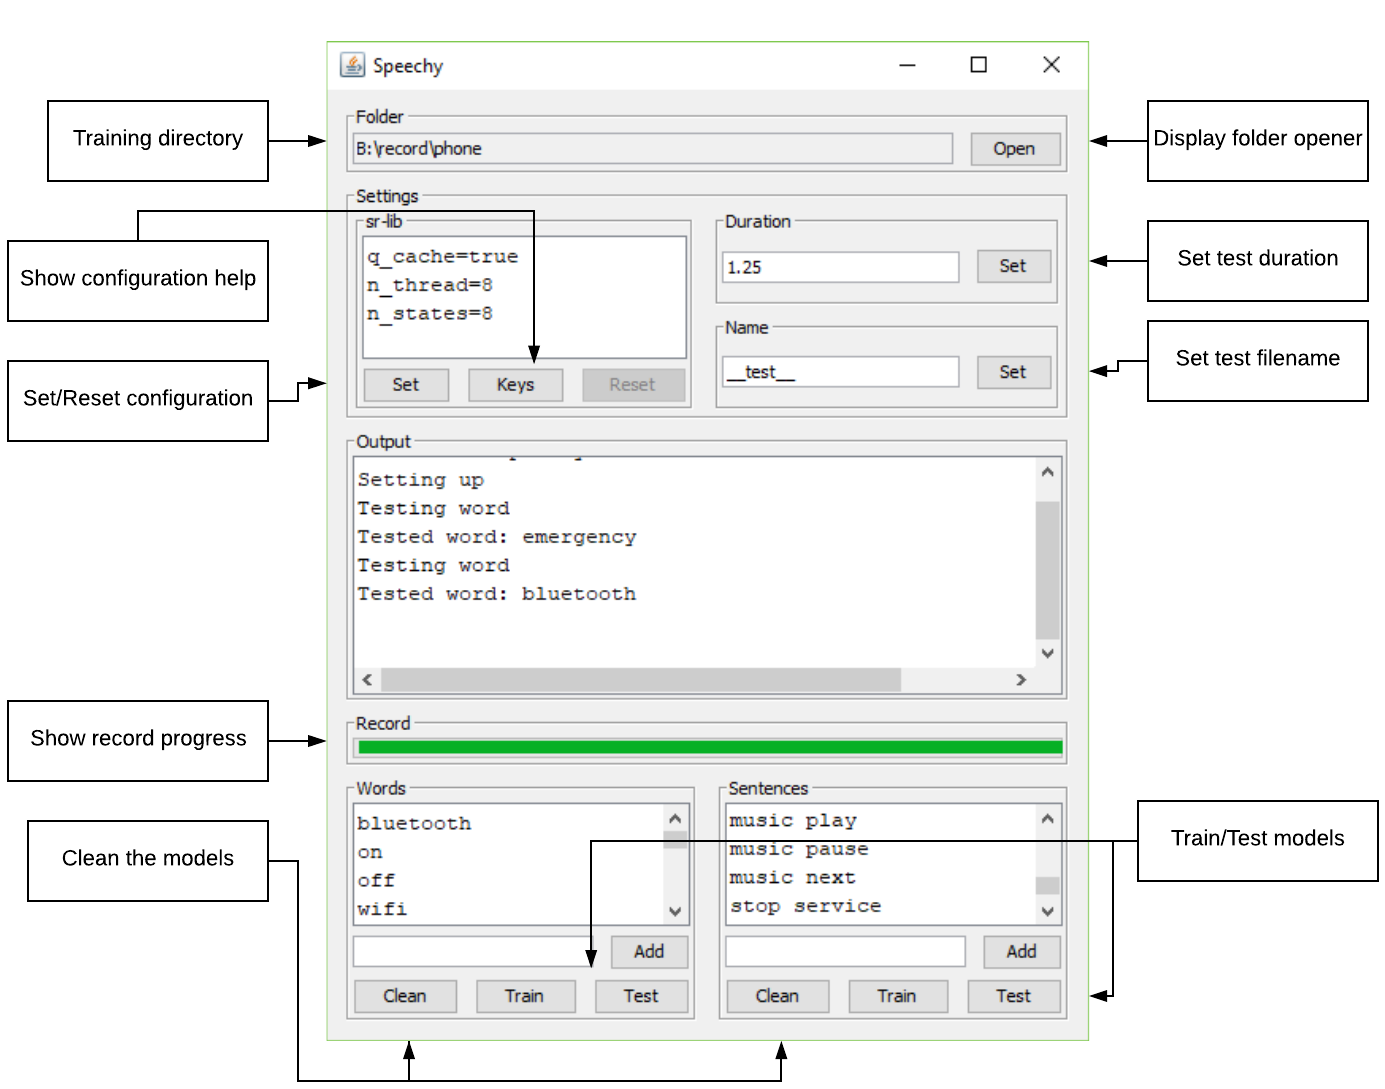
\includegraphics[scale=0.85]{desktop-screenshot}
    \label{fig:desktop-screenshot}
    \caption{Graphics User Interface for Training}
\end{figure}

\newpage

The interface has been made intuitive. Buttons are enabled only when required. For example, Test and Clean button will not be available until training is finished. At any moment only one task can be performed from the interface, and data race conditions between GUI and IO are avoided. The system is completely asynchronous and does not block the user interface.

\section{Voice Controlled Assistant for Android}

The android application is written in Kotlin and uses the Android NDK to run the speech recognition library.
The design of this application is inspired by Facebook Messenger chat heads. The main button is controlled by a service class that runs in the background. The main button is completely movable over the screen. It displays a round progress bar of the recording being done. A single click on the button starts recording for a sentence and user is expected to speak. A message toast is shown with every recognized word. If the recognition results match the list of actions, the corresponding action is performed. Currently, the application supports the following actions:
\begin{itemize}
    \item Open applications
    \item Enable/disable Bluetooth
    \item Control music player
    \item Enable/disable Wi-Fi
    \item Make phone calls
    \item Control brightness        
    \item Enable/disable torch
    \item Control volume
\end{itemize}

\begin{figure}[h!]
    \centering
    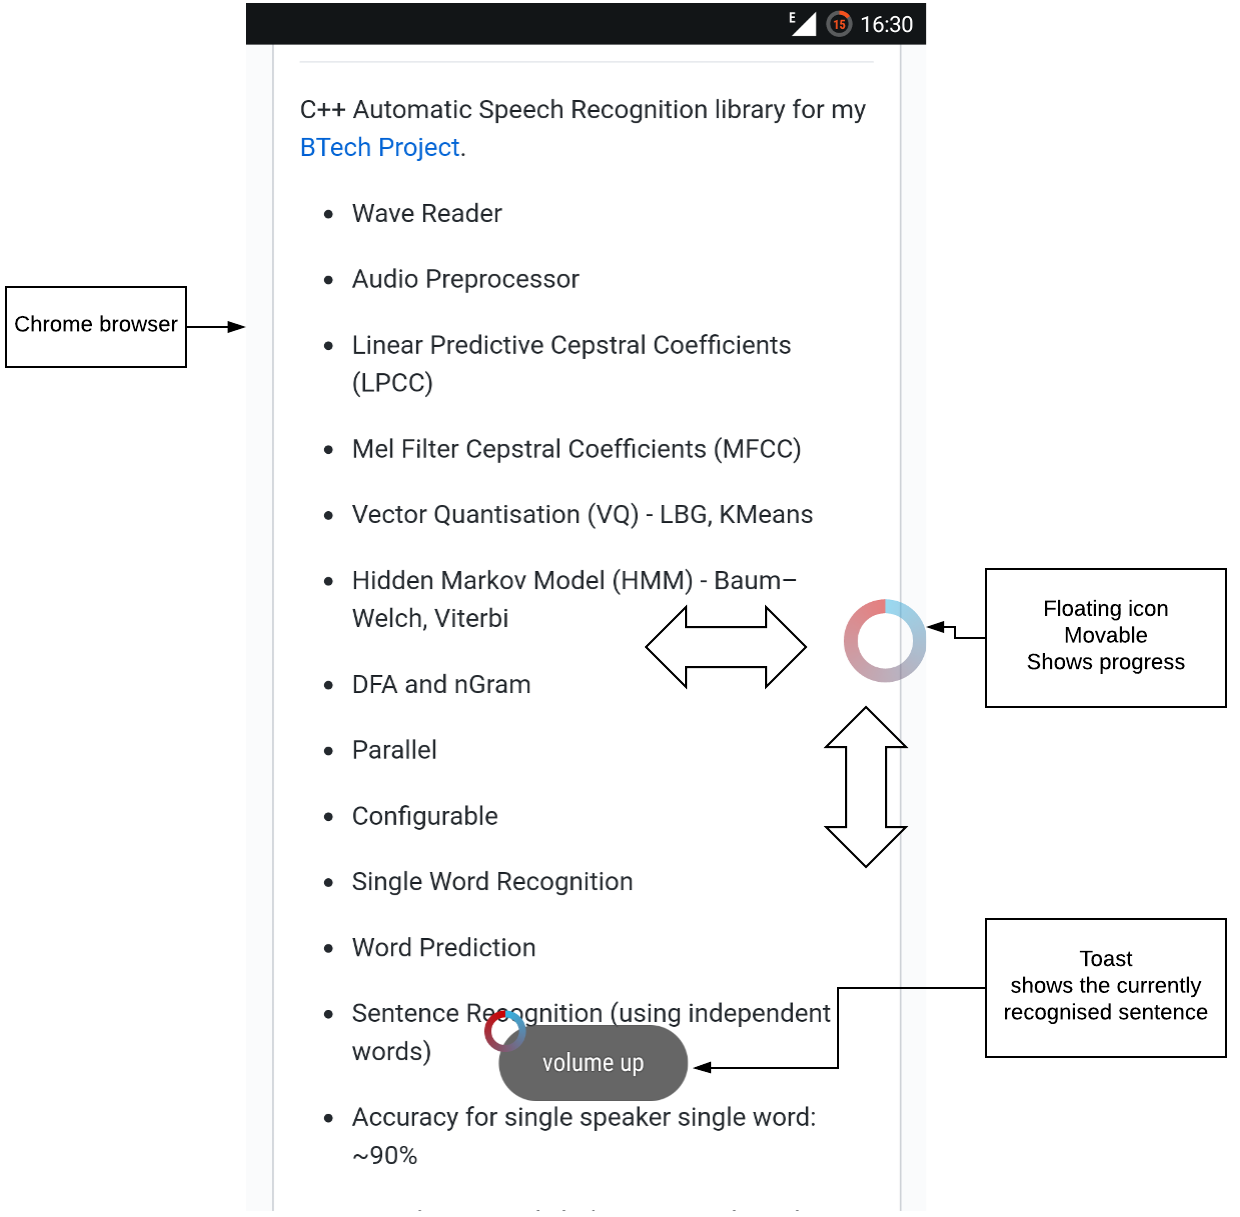
\includegraphics[scale=0.9]{android-screenshot}
    \label{fig:android-screenshot}
    \caption{Android Voice Controlled Assistant}
\end{figure}

The application makes extensive use of Kotlin’s co-routines to provide responsive GUI feedback. With the architecture of the application, more actions can be added with ease. To improve accuracy, the application also saves the recordings that are recognized so they can be trained by connecting to the desktop.

\chapter{Experiment and Observation} \label{ch:experiment}

We obtained a digits dataset with 15 utterances per digit, and a commands (for the android project) dataset with 25 utterances per word. The recordings were done in moderately quiet environments using a general-purpose microphone.

\begin{figure}
    \centering
    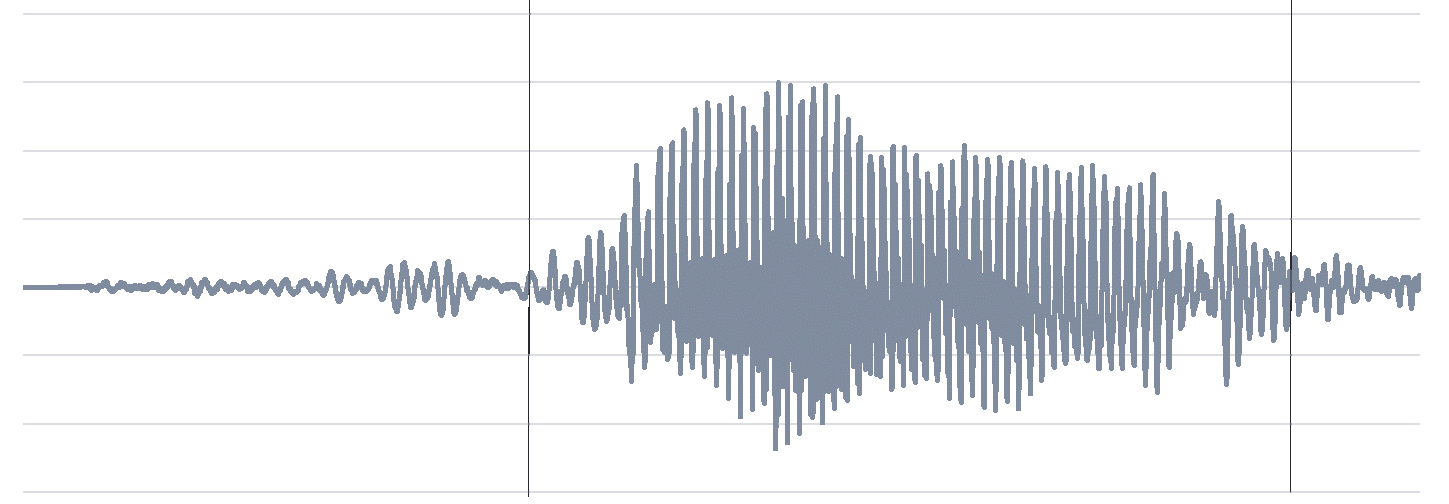
\includegraphics[scale=0.45]{graph-nine-trim}
    \label{fig:graph-nine-trim}
    \caption{Automatic trimming of nine}
\end{figure}

For the obtained datasets, the trimming algorithm presented very accurate results. The results were close to 88\% for the error of speech signal's endpoints missing by 100ms.

\newpage

\begin{figure}
    \centering
    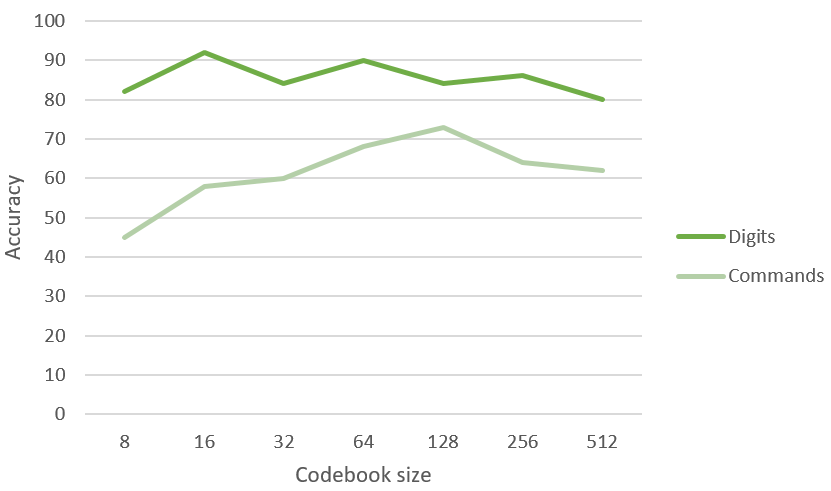
\includegraphics[scale=0.5]{graph-codebook-size}
    \label{fig:graph-codebook-size}
    \caption{Codebook size vs Accuracy}
\end{figure}

\begin{figure}
    \centering
    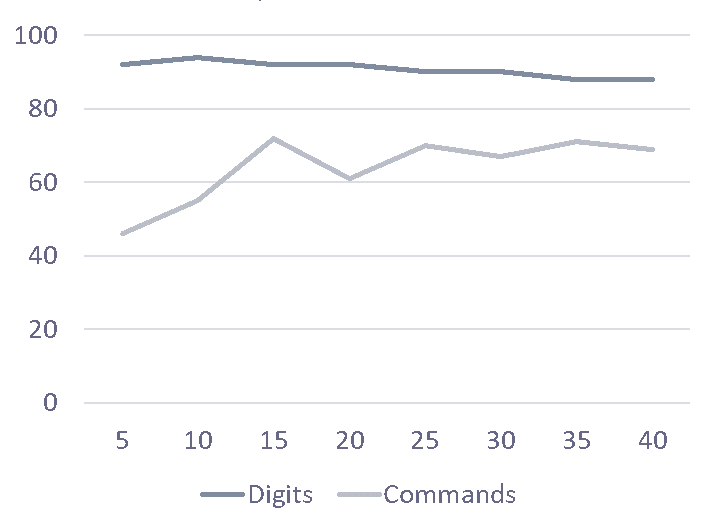
\includegraphics[scale=0.5]{graph-hidden-states}
    \label{fig:graph-hidden-states}
    \caption{Number of hidden states vs Accuracy}
\end{figure}

MFCC features resulted in better accuracy than LPCC features as expected. The accuracy of digits dataset decreased if delta or acceleration features were added, while it increased for commands dataset. The optimal codebook size and number of HMM states were higher for commands dataset than compared to digits dataset. Moreover, initial Bakis model with more jumps improved the performance for commands dataset.

\hfill

\begin{table}[H]
    \centering
    \begin{tabular}{lll}
    \hline
    Description           & Digits dataset & Commands dataset \\
    \hline
    Number of words       &  10     & 21 \\
    Number of utterances  &  150    & 525 \\
    \hline
    Delta features        &  No     & Yes \\
    Delta delta feautres  &  No     & Yes \\
    Codebook size         &  16  & 128 \\
    Number of hidden states  &  10 & 15 \\
    Jumps allowed in Bakis &  1 & 3 \\
    \hline
    Training time (s)     &  3.3 & 7.4 \\
    Accuracy (\%)         &  94 & 73 \\
    \hline
    \end{tabular}
    \caption{Results of speech recognition}
\end{table}   

For profiling the library on a desktop, Visual Studio Profiler was used and a Intel Corei7 3.0GHz + 8GB RAM laptop was selected. During training, the maximum CPU usage increased up to 80\% while the maximum RAM usage was below 20MB for our datasets.

For profiling the android application, Android Studio Profiler was used and an octa-core 1.7GHz + 2GB RAM mobile phone was selected. During testing, the maximum CPU usage increased up to 50\% while the RAM stayed constant at 12MB. The average recognition time for input utterances was 15ms.

It was observed that the system was not accurate enough for speaker independent scenarios with accuracy as low as 40\%. Noisy environments, changes in pitch and accents, similar sounding words in the dataset, and improper training parameters also reduced the accuracy of the system.
\chapter{Conclusion and Future Work} \label{ch:conclusion}

Our speech recognition system gave satisfactory accuracy while also being real-time. It works well even with less amounts of training data. It can be used to make simple recognition systems for individual persons and command based devices like wheelchairs or home automation systems. With time, our system can be trained on the previously recognized recordings to improve the performance.

Word recognition systems are easier to train and perform exceptionally well for simple tasks with less number of words.
With increase in number of words though, the execution becomes slow as there are more models to match. Hence, word based speech recognition systems are not suitable for large vocabulary systems. For future work, a phoneme based recognition system like tri-phone system can be added to the library.

The graphical user interface was very helpful for training. Feature for automatically dividing the dataset into train and test sets, and then finding accuracy can be added to the interface. Moreover, a brute-force approach can be used to select parameters like codebook size and number of HMM states from a set of pre-chosen values. The android application can be improved significantly by adding more actions and an artificial voice feedback.

\bibliography{references}
\bibliographystyle{alpha}

\appendix

\chapter{Preprocessing}
\subsubsection{Normalization}
This step is done to avoid the variations in amplitude between sound recordings from different devices.
\begin{equation*} x_i = x_i - x_{mean} \end{equation*}

\subsubsection{Trimming}
This step is necessary to save computational resources from being spent on unvoiced parts of the signal. Hence, silent parts of the signal should be removed. The trimming is done using the algorithm in \cite{Saha_anew}. This algorithm uses the background noise features to set thresholds, hence no need to assume any ad-hoc values. If $d$ (Mahalanobis distance) of a sample comes out to be lesser than 3, it is rejected. $b_{mean}, b_{sd}$ are the Gaussian parameters of the background noise.
\begin{equation*} d = x - b_{mean} / b_{sd} \end{equation*}

\newpage

\subsubsection{Pre-emphasis}
Due to the nature of the glottal impulse, the human speech has more energy in the lower frequencies. Hence, the signal is applied with pre emphasis filter (a first order high pass filter) that boosts the higher frequencies.
\begin{equation*} x_i = x_i - \alpha x_{i-1} \end{equation*}

This enables the acoustic models to gain more information from the higher formants. $\alpha = 0.95$ has been taken for our system. 

\subsubsection{Framing and Hamming Window}
We want to extract features from a small window of speech that represents a sub phoneme. To convert the signal to a stationary signal frame wise, a hamming window is applied on each frame. It disallows discontinuity by suppressing the boundaries of the signal. One of the most commonly used hamming window is:

\begin{equation*} w(i) = 0.54 - 0.46\frac{2\pi(i - 1)}{N - 1}, \quad \begin{aligned} 1 \leq i \leq N \end{aligned}
\end{equation*}

\chapter{Feature Extraction}
\section{LPCC}

Linear Predictive Coding is a very useful technique for encoding high quality speech at a low bit rates. It provides very accurate estimates of the speech parameters. Its main advantage comes from the fact that it is based on a simplified vocal tract model. LPC includes a speech production function mimicking the air from our lungs, and the error filter mimicking our larynx.

We find out the linear predictive cepstral coefficients (LPCC) using the autocorrelation method from \cite{rabinerbook}.

\subsubsection{Autocorrelation}
The first step is to find $p$ autocorrelation values for each frame of windowed signal using 

\begin{equation*} \sum_{n=0}^{n-1-m}{\tilde{x}_l(n)}{\tilde{x}_l(n+m)}, \quad \begin{aligned} m=0,1,...,p. \end{aligned} \end{equation*} 

$p$ is the linear prediction order.

\subsubsection{Durbin solve}
A $pXp$ Toeplitz matrix is created by using the above $p$ autocorrelation values. The Toeplitz matrix is solved using Durbin method to give the LPC coefficients:

\begin{equation*} E^{(0)} = R(0) \end{equation*}
\begin{equation*} k_i = \dfrac{R(i) - \sum_{j=1}^{i-1}\alpha_j^{i-1}R(|i-j|)}{E^{i-1}},  \quad \begin{aligned} 1 \leq i \leq p. \end{aligned} \end{equation*}
\begin{equation*} \alpha_i^{(i)} = k_i \end{equation*}
\begin{equation*}\alpha_j^{(i)} = \alpha_i^{(i-1)} - k_i\alpha_{i-1}^{(i-1)},   \quad \begin{aligned} 1 \leq j \leq i-1. \end{aligned}\end{equation*}
\begin{equation*} E^{i} = (1-k_i^2)E^{i-1} \end{equation*}

\begin{figure}[h!]
    \centering
    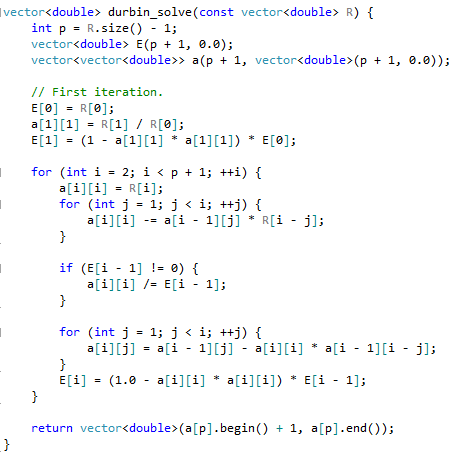
\includegraphics[scale=0.9]{sr-lib-durbin-code}
    \label{fig:sr-lib-durbin-code}
    \caption{Implementation of Durbin's solve}
\end{figure}

\subsubsection{Cepstral Coefficients}
In the last step, the LPC cepstral coefficients are derived from the LPC coefficients. $\sigma^2$ is the gain term of the LPC model.

\begin{equation*}
    c_0 = ln\sigma^2
\end{equation*}
\begin{equation*}
    c_m = a_m + \sum_{k = 1}^{m - 1}(\frac{k}{m})c_ka_{m-k}, 
    \quad \begin{aligned} 1 \leq m \leq p. \end{aligned}
\end{equation*}
\begin{equation*}
    c_m = \sum_{k = 1}^{m - 1}(\frac{k}{m})c_ka_{m-k}, 
    \quad \begin{aligned} m > p. \end{aligned}
\end{equation*}

LPCC are proved to be more robust than LPC. A sine window is applied over these cepstral coefficients to desensitize them towards noise and noise like sounds.

\section{MFCC}

MFCC is one of the most popular feature extraction technique. MFCC aims to mimic the human hearing by penalizing higher frequencies and boosting lower frequencies. The mapping between Hertz and Mel is logarithmic above 1000Hz and linear below 1000 Hz. The Mel scale is based on an empirical study conducted by Stevens and Volkmann.

\begin{equation*} m = 2595 log_10 (1 + \frac{f}{700}) \end{equation*}

\subsubsection{DFT}
The frequency spectrum is extracted by finding the Discrete Fourier Transform (using FFT) of each frame. We implement the FFT using Cooley-Tukey, in-place, breadth-first, decimation-in-frequency algorithm described in \cite{Blahut:1985:FAD:537283}.

\begin{figure}[h!]
    \centering
    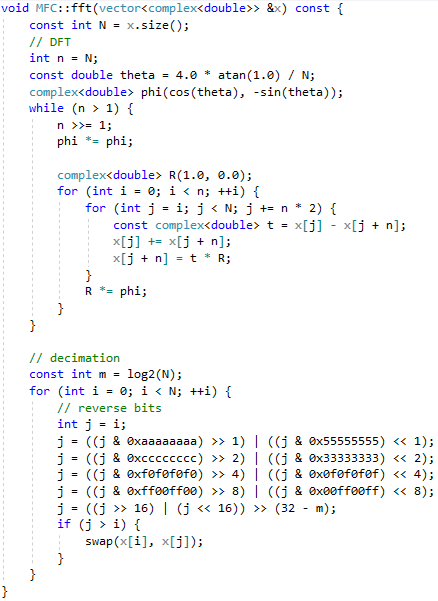
\includegraphics[scale=0.9]{sr-lib-fft-code}
    \label{fig:sr-lib-fft-code}
    \caption{Implementation of FFT}
\end{figure}

\subsubsection{LMFB}
This step is performed by using filter banks with filters centered according to the Mel frequencies.  We have used 40 filter banks in our implementation.

\subsubsection{DCT}

Inverse Fourier Transform is done using Discrete Cosine Transform in this step. The result of this step are the Mel frequency cepstral coefficients.

\begin{equation*}
    c[m] = \sum_{i=1}^M logY(i)cos[\frac{m\pi}{M}(i - 0.5)]
\end{equation*}

$M$ is the number of filters, $c[m]$ are the cepstral coefficients, $Y(i)$ are the filter outputs.

\subsubsection{Normalization}

To reduce the channel effect of the recordings, cepstral mean subtraction is done. When people record from different channels, different channel effect is created. $Q$ is the number of cepstral coefficients.

\begin{equation*}
    c_i = c_i - c_{mean},
    \quad \begin{aligned} 1 \leq i \leq Q. \end{aligned}
\end{equation*}

\section{Derivative coefficients}

Co-articulation and irregularities in speech cause the speech signal to not be stationary frame to frame. To acknowledge this delta and delta delta (acceleration) features can be calculated from the cepstral coefficients.
We use the linear regression method to calculate the derivative features.

\begin{equation*}
    \Delta c_j[i] = \frac{\sum_{m=-M}^{M} m c_{j+m}[i]}{\sum_{m=-M}^{M} m_2 }
\end{equation*}

Now the complete feature set is:
{\begin{itemize}
\item Q cepstral coefficients (using LPCC or MFCC)
\item Q delta cepstral coefficients
\item Q acceleration cepstral coefficients    
\end{itemize}}

\chapter{Vector Quantization}

Vector Quantization was originally being used for data compression, but it performs well even for speech recognition. A large set of vectors are divided into groups such that they have almost equal number of neighbors closest to them. VQ vastly decreases the data that has to be processed. Instead of having full utterances and words as training data, we will be able to have only a small sized codebook.

\section{KMeans}
KMeans is one of the most basic and yet useful algorithm or clustering of data. The algorithm is described as:

\begin{enumerate}
\item Choose N random points as centroids
\item Assign all other points to one of the N centroids based on distance
\item Recalculate the centroids by using the above created buckets
\item Repeat from step 2 till the centroids converge
\end{enumerate}

\section{LBG}
Linde Buzo Gray algorithm solves one of the very important shortcomings of KMeans. It solves the initialisation problem. KMeans chooses N random points and can reach local optimal states. To overcome this LBG algorithm completely removing initial randomness by using the following steps:

\begin{enumerate}
    \item Start with number of centroids as 1 (the mean of all vectors)
    \item Split the centroids into two
    \item Optimize the centroids using KMeans
    \item Repeat from step 2 till the desired size of centroids is reached
\end{enumerate}

\chapter{Word Modeling}

Now the feature extraction is done on input signals and then using the codebook, the closest bucket is found for each frame. This greatly reduces the amount of data that we have to process. These bucket values are referred to as the observations. HMM has a number of hidden states. The probability of being in a state at the beginning is given by the initial state distribution. Each state can output one observation with probability given by the output probability matrix. Reaching one state from another has the probability given in transition probability matrix. 

Hidden Markov Models defines three basic problem:

\begin{enumerate}
    \item Evaluation problem

    Given a model and a sequence of observations, find the probability that the observations were generated by this model. This corresponds to recognizing the given input signal. Models for all words will be created and the model that gives the highest probability is the recognized word.

    \item Decoding problem

    Given a model and a sequence of observations, find the most optimal state sequence that produced given observations.

    \item Learning problem

    Given a model and a sequence of observations, how to adjust the model so it maximizes the probability from the Evaluation Problem. This corresponds to training the models on the given dataset. Each model for a word will be trained on all the utterances of that word in the training data. The initial model taken is a feed forward model. In feed forward model, every state can jump to the states next to itself. The length of jumps can be limited.

\end{enumerate}

All implementations regarding HMM were implemented by referring to \cite{18626}. A model is defined by initial state distribution $\pi$, transition probabilities $A$, and output probabilities $B$.

Given states $S = S_1, S_2 ... S_N$, observations $O = O_1O_2...O_T$, and $\lambda = (A, B, \pi)$, and let the state sequence be $q = q_1q_2...q_T$.

\section{Forward Procedure}
Forward procedure solves the Evaluation problem. It uses a dynamic programming approach. Let $\alpha_t(i)$ be the forward probability variable at instant $t$ state $i$.

Formula:
\begin{equation*}
    \alpha_t(i) = P(O_1...O_t, q_t = S_i | \lambda)
\end{equation*}

Initialization:
\begin{equation*}
    \alpha_1(i) = \pi_i b_i (O_1)
    \quad \begin{aligned} 1 \leq i \leq N \end{aligned}
\end{equation*}

Induction:
\begin{equation*}
    \alpha_{t+1}(j) = [\sum_{i=1}^N \alpha_t(i)a_{ij}]b_j(O_{t+1})
    \quad \begin{aligned} 1 \leq t \leq T-1, 1 \leq i \leq N \end{aligned}
\end{equation*}

Termination:
\begin{equation*}
    P(O|\lambda) = \sum_{i=1}^{N} \alpha_T(i)
\end{equation*}

$P(O|\lambda)$ is the probability that the observations were generated by this model.

\section{Viterbi Algorithm}
Viterbi algorithm solves the Decoding problem. It also uses a dynamic programming approach. Let $\delta_t(i)$ be the delta probability variable at instant $t$ state $i$.

Formula:
\begin{equation*}
    \delta_t(i) = \max_{q_1, q_2 ... 1_{t-1}} P(q_1, q_2,...q_{t-1}, q_t = S_i, O_1O_2...O_t | \lambda)
\end{equation*}

Initialization:
\begin{equation*}
    \delta_1(i) = \pi_i b_i (O_1)
    \quad \begin{aligned} 1 \leq i \leq N \end{aligned}
\end{equation*}

\begin{equation*}
    \psi_1(i) = 0
\end{equation*}

Induction:
\begin{equation*}
    \delta_t(j) = \max_{i\leq i \leq N}[\delta_{t-1}(i)a_{ij}]b-J(O_t)
    \quad \begin{aligned} 2 \leq t \leq T \end{aligned}
\end{equation*}

\begin{equation*}
    \psi_t(j) = arg\max_{i\leq i \leq N}[\delta_{t-1}(i)a_{ij}]b-J(O_t)
    \quad \begin{aligned} 2 \leq t \leq T \end{aligned}
\end{equation*}

Termination:
\begin{equation*}
    P^* = \max_{1\leq i \leq N}[\delta_T(i)]
    q_T^* = arg\max_{1\leq i \leq N}[\delta_T(i)]
\end{equation*}

Backtracking the path:
\begin{equation*}
    q_t^* = \psi_{t+1}(q_{t+1}^*)
\quad \begin{aligned} T-1 \geq t \geq 1 \end{aligned}
\end{equation*}

$q^*$ is the optimal state sequence.

\section{Baum Welch Re-estimation}
Baum Welch re-estimation solves the Learning problem.

Backward procedure is a necessity for this algorithm. Backward procedure is similar to the forward procedure but the flow is in backward direction. Let $\beta_t(i)$ be the probability variable at instant $t$ state $i$.

Formula:
\begin{equation*}
    \beta_t(i) = P(O_{i+1}, O_{i+2}...O_T, q_t = S_i | \lambda)
\end{equation*}

Initialization:
\begin{equation*}
    \beta_T(i) = 1
    \quad \begin{aligned} 1 \leq i \leq N \end{aligned}
\end{equation*}

Induction:
\begin{equation*}
    \beta_t(i) = \sum_{j=1}^N a_{ij} b_j(O_{t+1}) \beta_{t+1}(j)
    \quad \begin{aligned} T > t \geq 1, 1 \leq i \leq N \end{aligned}
\end{equation*}

Now let us define $\gamma_t(i)$ as the probability of being in state i at instant t.

Formula:
\begin{equation*}
    \gamma_t(i) = P(q_t = S_t | O, \lambda)
    \gamma_t(i) = P(O, q_t = S_i | \lambda)
    \gamma_t(i) = \frac{\alpha_t(i) \beta_t(i)}{\sum_{i=1}^N\alpha_t(i) \beta_t(i)} 
\end{equation*}

Let $\xi_t(i,j)$ as the probability of being in state $i$ at time $t$ and going to state $j$ at time $t+1$.

Formula:
\begin{equation*}
    \xi_t(i,j) = P(q_t = S_i, q_{t+1} = S_j | O, \lambda)
\end{equation*}

Using forward and backward variables, we find:

\begin{equation*}
    \xi_t(i,j) = \frac{\alpha_t(i)a_{ij}b_j(O_{t+1}\beta_{t+1}(j))}{\sum_{i=1}^N \alpha_t(i) \beta_t(i)}
\end{equation*}

\begin{equation*}
    \gamma_t(i) = \sum_{j=1}^N \xi_t(i,j)
\end{equation*}

Calculation of new $\pi$:

\begin{equation*}
    \hat{\pi_i} = \text{expected number of times in state } S_i \text{ at time } t = 1
\end{equation*}

\begin{equation*}
    \hat{\pi_i} = \gamma_1(i)
\end{equation*}

Calculation of new $A$:

\begin{equation*}
    \hat{a_{ij}} = \frac{\text{expected number of transition from state $S_i$ to $S_j$}}{\text{expected number of transition from state $S_i$}}
\end{equation*}

\begin{equation*}
    \hat{a_{ij}} = \frac{\sum_{t=1}{T-1}\xi_t(i,j)}{\sum_{t=1}{T-1}\gamma_t(i)}
\end{equation*}

Calculation of new $B$:

\begin{equation*}
    \hat{b_{j}(k)} = \frac{\text{exptected number of times in state $S_j$ and observing output $V_k$}}{\text{expected number of times in state $S_j$}}
\end{equation*}

\begin{equation*}
    \hat{b_{j}(k)} = \frac{\sum_{t=1, O_t = V_k}^{T}\gamma_t(j)}{\sum_{t=1}^{T}\gamma_t(j)}
\end{equation*}

\section{Scaling and Tweaking}

As the number of observations increases, calculations of $\delta$, $\alpha$, $\beta$ head to very small numbers. These numbers cannot be represented even in double float precision. Hence scaling has to be performed.

For Viterbi algorithm, scaling can be avoided if all the calculations are done in log space. 

On the contrary, both forward and backward procedures involve summation of large number of terms. Therefore, log space cannot be used. To scale these procedures, scaling coefficients are used \cite{18626}.

To make up for the lack of infinite precision on the processors, tweaking has to be done of the model at each step of Baum Welch re-estimation. In the transition matrix and the output matrix, the probabilities that turn to zero are given a minimum probability value. This helps the model to learn well during training.

\chapter{Sentence Modeling}

Sentence modeling in our system is estimating probability of each word given its prior context. Example: $P(\text{off} | \text{turn torch})$

\section{NGram}

NGram is a (N-1) order Markov model. The Markov assumption is the presumption that future behavior of a dynamic system depends only on its recent history. 
NGram posterior probabilities can be found using the relative frequencies of words. This method is called Maximum Likelihood Estimation. Assume word sequence $w_1...w_n$ and $C$ is the count of the NGram.

\begin{equation*}
P(w_n|w_{n-N+1}^{n-1}) = \frac{C(w_{n-N+1}^{n-1} w_n)}{w_{n-N+1}^{n-1}}
\end{equation*}

This estimates the NGram probability by dividing the observed frequency of a particular sentence by the observed frequency of the prefix.

\section{DFA}

Deterministic Finite Automata for sentence modeling is created by adding a necessary initial point condition to the NGram generator. In the implementation, only the sentences that start from the initial word are counted. Hence, the formula for MLE remains the same.

Any sentence that do not follow the complete structure of sentences in the training is assigned zero probability. Hence, it can never occur as one of the recognized sentence.

\end{document}
